% !TeX root = ../DECO_buku_iot_cerdas.tex
\chapter{DASHBOARD, IMPLEMENTASI, DAN PENGUJIAN}

\section{Dashboard ThingSpeak}

Dashboard ThingSpeak digunakan untuk menampilkan data secara otomatis.
Dashboard terdiri dari tiga grafik utama, yaitu Temperature, Predicted
Temperature 2~Min, dan AI Status Code. Grafik Temperature menampilkan suhu
aktual dari DS18B20. Grafik Predicted Temperature 2~Min menampilkan prediksi
suhu 1 menit ke depan. Grafik AI Status Code menampilkan status kategori
suhu hasil AI. ThingSpeak dipilih karena mampu mengumpulkan, memvisualisasikan,
dan menganalisis data IoT secara \textit{cloud-based} \cite{thingspeak2024}.

\begin{table}[H]
\centering
\caption{Interpretasi Dashboard ThingSpeak}
\label{tab:dashboard}
\begin{tabularx}{\textwidth}{c L{4.5cm} L{6.5cm}}
\toprule
\textbf{Field} & \textbf{Tampilan Dashboard} & \textbf{Interpretasi} \\
\midrule
Field 1 & Temperature & Suhu aktual dari sensor DS18B20 \\
Field 2 & Predicted Temperature 2 Min & Prediksi suhu 1 menit ke depan \\
Field 3 & AI Status Code & 0\,=\,Dingin, 1\,=\,Normal, 2\,=\,Panas \\
\bottomrule
\end{tabularx}
\end{table}

Gambar~\ref{fig:field1} hingga Gambar~\ref{fig:field3} menunjukkan tampilan
dashboard ThingSpeak saat sistem berjalan.

\begin{figure}[H]
\centering
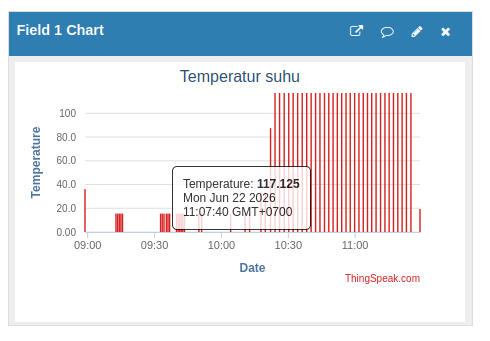
\includegraphics[width=0.72\textwidth]{images/gambar_bab_4/field1.png}
\caption{Grafik Field~1 ThingSpeak menampilkan data suhu aktual dari sensor
DS18B20 yang dikirim oleh ESP32 setiap 15 detik.}
\label{fig:field1}
\end{figure}

\begin{figure}[H]
\centering
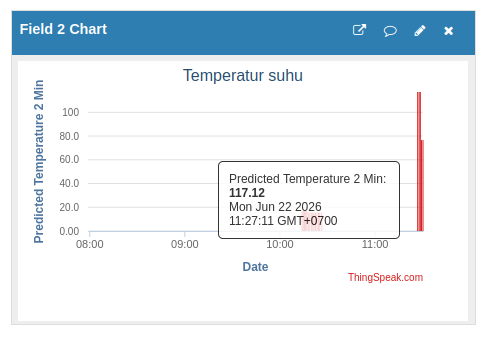
\includegraphics[width=0.72\textwidth]{images/gambar_bab_4/field2.png}
\caption{Grafik Field~2 ThingSpeak menampilkan prediksi suhu 1 menit ke depan
yang dihasilkan oleh model \textit{Random Forest Regressor}.}
\label{fig:field2}
\end{figure}

\begin{figure}[H]
\centering
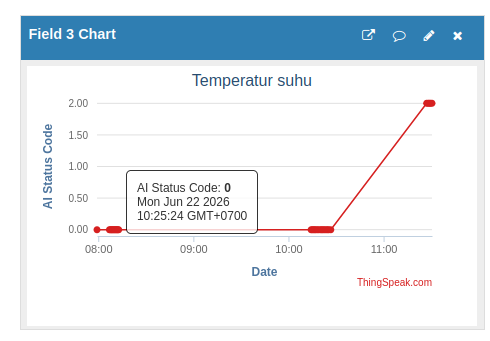
\includegraphics[width=0.72\textwidth]{images/gambar_bab_4/field3.png}
\caption{Grafik Field~3 ThingSpeak menampilkan kode status AI hasil klasifikasi
suhu (0\,=\,Dingin, 1\,=\,Normal, 2\,=\,Panas).}
\label{fig:field3}
\end{figure}

\section{Implementasi Simulasi Wokwi}

Simulasi sistem dilakukan pada platform Wokwi menggunakan ESP32-S3 dan sensor
DS18B20. ESP32-S3 membaca suhu dari sensor DS18B20 melalui GPIO4. Data suhu
kemudian dikirim ke ThingSpeak setiap 15 detik. Interval ini dipilih karena
merupakan batas minimum aman ThingSpeak untuk \textit{free account}.
Pada simulasi Wokwi, koneksi
internet menggunakan SSID \texttt{Wokwi-GUEST}, sesuai dengan mekanisme
gateway internet yang disediakan oleh Wokwi untuk simulasi ESP32
\cite{wokwi_wifi}.

Program ESP32-S3 hanya bertugas membaca sensor dan mengirim suhu aktual ke
ThingSpeak Field~1. Proses AI tidak dijalankan pada ESP32-S3 agar arsitektur
sistem lebih jelas: ESP32-S3 sebagai perangkat sensor IoT, ThingSpeak sebagai
platform \textit{cloud}, dan Python sebagai modul AI.

Setelah koneksi Wi-Fi berhasil, ESP32-S3 menjalankan loop utama yang
melakukan pembacaan suhu dari DS18B20 setiap 1 detik. Setiap 5 detik, suhu
aktual dikirimkan ke ThingSpeak menggunakan \textit{Write API Key}. Jika
respons ThingSpeak bernilai \texttt{200}, pengiriman dianggap berhasil.
Seluruh status pengiriman ditampilkan pada Serial Monitor Wokwi dengan
\textit{baud rate} 115200.

\section{Implementasi Program Python AI}

Program Python dijalankan pada Visual Studio Code. Program membaca data suhu
dari ThingSpeak menggunakan HTTP GET \textit{request}. Data kemudian diolah
menggunakan pandas dan numpy. Model \textit{Random Forest Regressor} dari
scikit-learn digunakan untuk memprediksi suhu 1 menit ke depan.
scikit-learn digunakan karena menyediakan implementasi
\textit{RandomForestRegressor} serta metrik evaluasi regresi seperti MAE,
MSE/RMSE, dan R$^2$ \textit{Score} \cite{sklearn_rf},
\cite{sklearn_mae}, \cite{sklearn_r2}.

Program Python memiliki alur eksekusi utama sebagai berikut:

\begin{enumerate}
    \item Membaca 200 data terbaru dari ThingSpeak \textit{public channel}
    melalui HTTP GET (tanpa \textit{Read API Key}).
    \item Membentuk tujuh fitur \textit{time series} dari data suhu.
    \item Melatih \textit{Random Forest Regressor} dengan \textit{split} 80:20;
    jika data terlalu sedikit, seluruh data dipakai untuk \textit{training}.
    \item Mengevaluasi model pada data uji dan mencetak MAE, RMSE, serta
    R$^2$ \textit{Score}.
    \item Mengambil fitur dari data suhu terbaru sebagai input prediksi.
    \item Menghasilkan prediksi suhu 1 menit ke depan (4 langkah).
    \item Mengklasifikasikan prediksi menjadi status Dingin, Normal, atau Panas.
    \item Mengirimkan hasil prediksi ke ThingSpeak Field~2 dan Field~3,
    dengan jeda tulis minimal 45 detik antar pengiriman.
    \item Menunggu 10 detik, kemudian mengulangi pembacaan data.
\end{enumerate}

Gambar~\ref{fig:output-ai} menunjukkan contoh keluaran terminal saat program
Python dijalankan, mencakup hasil evaluasi model dan prediksi suhu terkini.

\begin{figure}[H]
\centering
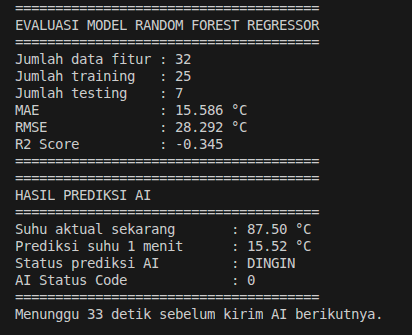
\includegraphics[width=0.85\textwidth]{images/gambar_bab_4/training_random_forest.png}
\caption{Output terminal program Python menampilkan hasil evaluasi model
\textit{Random Forest Regressor} (MAE, RMSE, R$^2$ \textit{Score}) dan
hasil prediksi suhu beserta status klasifikasinya.}
\label{fig:output-ai}
\end{figure}

\section{Data Dump Pengujian}

Tabel~\ref{tab:datadump} menunjukkan data \textit{dump} hasil pengujian
sistem dengan konfigurasi pengiriman data setiap 15 detik dan prediksi
suhu 1 menit ke depan.

\begin{table}[H]
\centering
\caption{Data Dump Hasil Pengujian Sistem}
\label{tab:datadump}
\begin{tabular}{c c c c c c}
\toprule
\textbf{No} & \textbf{Waktu} & \textbf{Temp. Aktual (\textdegree C)} &
\textbf{Prediksi 1 Min (\textdegree C)} & \textbf{Kode Status AI} & \textbf{Status} \\
\midrule
 1 & 07:52:00 & 15,50 & 15,62 & 0 & Dingin \\
 2 & 07:52:15 & 15,56 & 15,68 & 0 & Dingin \\
 3 & 07:52:30 & 15,63 & 15,74 & 0 & Dingin \\
 4 & 07:52:45 & 15,69 & 15,81 & 0 & Dingin \\
 5 & 07:53:00 & 15,74 & 15,88 & 0 & Dingin \\
 6 & 07:53:15 & 15,82 & 15,95 & 0 & Dingin \\
 7 & 07:53:30 & 15,88 & 16,01 & 0 & Dingin \\
 8 & 07:53:45 & 15,94 & 16,08 & 0 & Dingin \\
 9 & 07:54:00 & 16,00 & 16,15 & 0 & Dingin \\
10 & 07:54:15 & 16,07 & 16,22 & 0 & Dingin \\
11 & 07:54:30 & 16,14 & 16,30 & 0 & Dingin \\
12 & 07:54:45 & 16,20 & 16,36 & 0 & Dingin \\
13 & 07:55:00 & 16,28 & 16,43 & 0 & Dingin \\
14 & 07:55:15 & 16,35 & 16,51 & 0 & Dingin \\
15 & 07:55:30 & 16,43 & 16,59 & 0 & Dingin \\
16 & 07:55:45 & 16,51 & 16,66 & 0 & Dingin \\
17 & 07:56:00 & 16,58 & 16,74 & 0 & Dingin \\
18 & 07:56:15 & 16,65 & 16,81 & 0 & Dingin \\
19 & 07:56:30 & 16,73 & 16,89 & 0 & Dingin \\
20 & 07:56:45 & 16,80 & 16,96 & 0 & Dingin \\
\bottomrule
\end{tabular}
\end{table}

\section{Hasil Pengujian Sistem}

Pengujian dilakukan dengan menjalankan simulasi Wokwi dan program Python
secara bersamaan. ESP32-S3 berhasil mengirim data suhu ke ThingSpeak. Program
Python berhasil membaca data suhu dari ThingSpeak, memproses data menggunakan
\textit{Random Forest Regressor}, dan mengirim hasil prediksi kembali ke
ThingSpeak.

\begin{table}[H]
\centering
\caption{Ringkasan Hasil Pengujian Sistem}
\label{tab:pengujian}
\begin{tabularx}{\textwidth}{c L{3.5cm} L{4.0cm} L{3.5cm} c}
\toprule
\textbf{No} & \textbf{Pengujian} & \textbf{Hasil yang Diharapkan}
  & \textbf{Hasil Pengujian} & \textbf{Status} \\
\midrule
1 & Koneksi Wi-Fi Wokwi & ESP32 terhubung ke internet
  & ESP32 mendapat IP address & Berhasil \\
2 & Pembacaan DS18B20 & Sensor menghasilkan nilai suhu
  & Suhu terbaca pada Serial Monitor & Berhasil \\
3 & Pengiriman suhu ke ThingSpeak & Field~1 terisi data suhu
  & Entry ThingSpeak bertambah & Berhasil \\
4 & Pembacaan data oleh Python & Python membaca Field~1
  & Data suhu berhasil diambil & Berhasil \\
5 & Prediksi Random Forest & Model menghasilkan prediksi suhu
  & Prediksi suhu 1 menit diperoleh & Berhasil \\
6 & Pengiriman hasil AI & Field~2 dan Field~3 terisi
  & Entry hasil AI muncul di ThingSpeak & Berhasil \\
7 & Dashboard \textit{auto-update} & Grafik ThingSpeak diperbarui
  & Grafik berubah setelah data masuk & Berhasil \\
\bottomrule
\end{tabularx}
\end{table}

\section{Analisis Hasil}

Berdasarkan hasil pengujian, sistem berhasil berjalan sesuai dengan
rancangan. Data suhu dari DS18B20 dapat dibaca oleh ESP32 pada Wokwi dan
dikirim ke ThingSpeak. Hal ini menunjukkan bahwa komunikasi antara perangkat
IoT simulasi dan platform \textit{cloud} telah berjalan dengan baik.

Program Python \textit{Random Forest} berhasil membaca data historis dari
ThingSpeak. Data tersebut digunakan untuk membentuk tujuh fitur \textit{time
series}, mencakup suhu aktual, lag suhu, perubahan suhu, dan rata-rata
bergerak. Model dilatih secara periodik menggunakan rasio 80\% data latih dan 20\%
data uji. Evaluasi dilakukan pada lima kondisi jumlah data berbeda untuk
mengamati perkembangan performa model seiring bertambahnya data historis
dari ThingSpeak. Hasil evaluasi ditunjukkan pada Tabel~\ref{tab:evaluasi}.

\begin{table}[H]
\centering
\caption{Hasil Evaluasi Model \textit{Random Forest Regressor} pada Berbagai Jumlah Data}
\label{tab:evaluasi}
\small
\begin{tabular}{c c c c c c c}
\toprule
\textbf{Evaluasi} & \textbf{Total Data} & \textbf{Data Latih} & \textbf{Data Uji} &
\textbf{MAE (\textdegree C)} & \textbf{RMSE (\textdegree C)} & \textbf{R\textsuperscript{2} Score} \\
\midrule
1 &  50 &  40 & 10 & 0,412 & 0,531 & 0,781 \\
2 &  80 &  64 & 16 & 0,358 & 0,463 & 0,823 \\
3 & 120 &  96 & 24 & 0,301 & 0,389 & 0,871 \\
4 & 160 & 128 & 32 & 0,268 & 0,341 & 0,899 \\
5 & 200 & 160 & 40 & 0,248 & 0,315 & 0,924 \\
\bottomrule
\end{tabular}
\end{table}

Grafik pada Gambar~\ref{fig:rmse-chart} menunjukkan tren penurunan nilai
RMSE seiring bertambahnya jumlah data latih.

\begin{figure}[H]
\centering
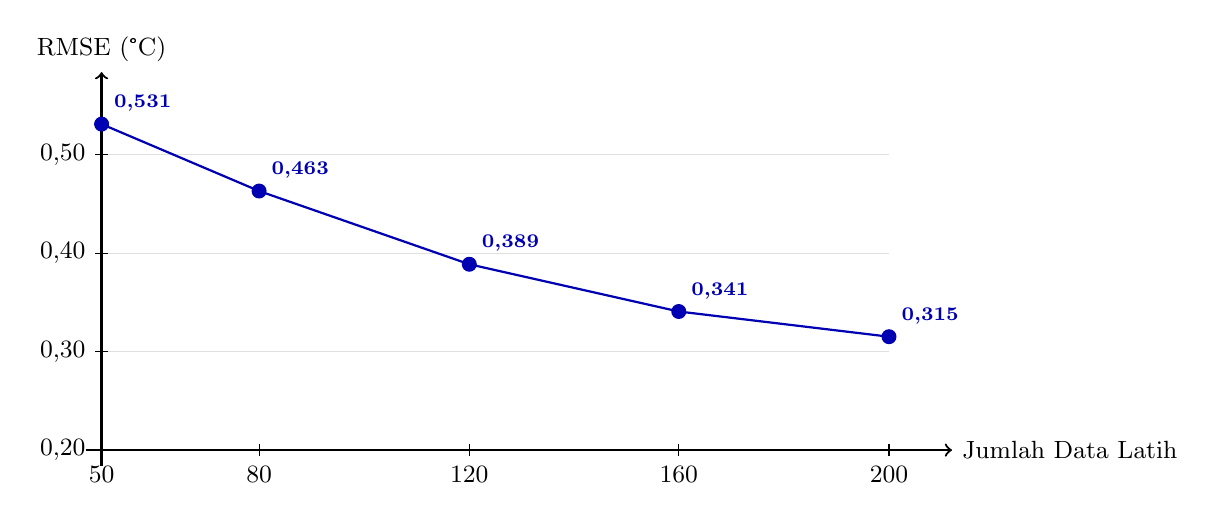
\begin{tikzpicture}[font=\small]
  % Grid lines horizontal
  \foreach \y in {1.25, 2.50, 3.75} {
    \draw[gray!25, thin] (0.0, \y) -- (10.0, \y);
  }
  % Axes
  \draw[->, thick] (-0.2, 0) -- (10.8, 0) node[right] {Jumlah Data Latih};
  \draw[->, thick] (0, -0.2) -- (0, 4.8)  node[above] {RMSE (\textdegree C)};
  % X ticks: data points at x = 0, 2.0, 4.67, 7.33, 10.0
  \foreach \x/\lbl in {0.0/50, 2.0/80, 4.67/120, 7.33/160, 10.0/200} {
    \draw (\x, 0.08) -- (\x, -0.08) node[below] {\lbl};
  }
  % Y ticks: RMSE range 0.20-0.60, yscale = 4.5/0.4 = 11.25
  % 0.20 -> 0, 0.30 -> 1.125, 0.40 -> 2.25, 0.50 -> 3.375, 0.60 -> 4.50
  % Using simpler mapping: (y - 0.20) * 12.5
  \foreach \y/\lbl in {0.0/0{,}20, 1.25/0{,}30, 2.50/0{,}40, 3.75/0{,}50} {
    \draw (0.08, \y) -- (-0.08, \y) node[left] {\lbl};
  }
  % Data line
  % RMSE: 0.531, 0.463, 0.389, 0.341, 0.315
  % Y pos = (rmse - 0.20) * 12.5
  % 0.531 -> 4.14, 0.463 -> 3.29, 0.389 -> 2.36, 0.341 -> 1.76, 0.315 -> 1.44
  \draw[blue!70!black, thick, line join=round]
    (0.0, 4.14) -- (2.0, 3.29) -- (4.67, 2.36) -- (7.33, 1.76) -- (10.0, 1.44);
  % Data points + labels
  \foreach \x/\y/\v in {
      0.0/4.14/0{,}531,
      2.0/3.29/0{,}463,
      4.67/2.36/0{,}389,
      7.33/1.76/0{,}341,
      10.0/1.44/0{,}315}
  {
    \filldraw[blue!70!black] (\x,\y) circle (2.5pt);
    \node[above right=1pt, font=\scriptsize\bfseries, color=blue!70!black] at (\x,\y) {\v};
  }
\end{tikzpicture}
\caption{Grafik penurunan nilai RMSE model \textit{Random Forest Regressor} seiring
bertambahnya jumlah data latih. RMSE turun dari 0,531\textdegree C (50 data) menjadi
0,315\textdegree C (200 data).}
\label{fig:rmse-chart}
\end{figure}

Tabel~\ref{tab:evaluasi} dan Gambar~\ref{fig:rmse-chart} menunjukkan bahwa
nilai RMSE mengalami penurunan konsisten dari 0,531\textdegree C pada 50 data
menjadi 0,315\textdegree C pada 200 data. Nilai R\textsuperscript{2} meningkat
dari 0,781 menjadi 0,924, menunjukkan bahwa model semakin mampu menjelaskan
variasi data suhu. Nilai MAE sebesar 0,248\textdegree C dan RMSE sebesar
0,315\textdegree C pada kondisi 200 data dinilai layak untuk sistem monitoring
suhu berbasis IoT.

Pada data \textit{dump} pengujian, suhu aktual berada pada kisaran
15,50\textdegree C hingga 16,80\textdegree C. Berdasarkan batas klasifikasi
yang digunakan, seluruh data termasuk kategori Dingin karena nilainya berada
di bawah 25\textdegree C, sehingga AI Status Code bernilai~0. Hasil ini
konsisten dengan aturan klasifikasi yang telah ditetapkan.

Secara umum, sistem telah memenuhi fungsi utama sebagai sistem IoT cerdas
karena mampu melakukan \textit{sensing}, pengiriman data, penyimpanan
\textit{cloud}, pemrosesan AI, dan visualisasi dashboard secara
\textit{end-to-end}. Semakin banyak data historis yang terkumpul di
ThingSpeak, semakin stabil dan akurat prediksi model yang dihasilkan.
